\chapter{Progettazione del cloud}

All'interno di questo capitolo verranno descritte quelle che sono state le scelte di progettazione del cloud riguardanti architettura hardware, metodologie di deployment e architettura di rete e i motivi per cui sono state fatte determinate scelte.

\section{Hardware}\label{subsec:progettazione_hardware}

L'hardware utilizzato per lo svolgimento di questa tesi è descritto in \cref{tab:hardware_inventory}.

\begin{table}[H]
    \caption{Hardware utilizzato per il progetto.}
\begin{center}
        \begin{tabular}{ |c|c| }
\hline
\textbf{Oggetto} & \textbf{Quantità}\\
\hline
Raspberry Pi 4 8 GB & 2\\
PC con architettura AMD64 & 6\\
HDD 1TB & 12\\
Switch layer 2 & 1\\
            Adattatore Ethernet USB & 1\\
            Cavi ethernet & 9\\
\hline
\end{tabular}
\end{center}
    \label{tab:hardware_inventory}
\end{table}

\noindent
Nello specifico i PC con architettura AMD64 hanno un processore Intel Core i5-4460S, 8 GB di RAM e due HDD da 1 TB ciascuno.
% 
Inizialmente uno solo dei due HDD era collegato alla scheda madre (il secondo era comunque già all'interno della macchina), quindi è stato necessario aprire ciascun computer e collegare gli hard disk alla scheda madre con un cavo SATA. 
% 
Per fare questo è stato necessario scollegare il lettore CD perché tutte le schede madri delle macchine a disposizione hanno solamente due porte SATA.

Il motivo per cui è stato necessario utilizzare due HDD su ciascuna macchina è che Ceph, ovvero il servizio che fornisce lo storage, necessita di un hard disk fisico dedicato per poter funzionare e non può condividerlo con il sistema operativo.

Per quanto riguarda i Raspberry Pi invece, era previsto di utilizzarne solamente uno ma, successivamente alla scelta della metodologia di deployment (descritta nella \cref{sec:deplyoment_method}), è stato deciso di utilizzarne uno aggiuntivo su cui installare MAAS, in modo da avere una macchina in più da poter dedicare effettivamente a OpenStack.

\section{Metodologia di deployment}\label{sec:deplyoment_method}

Nel momento in cui sono iniziati i lavori per questo progetto di tesi l'ultima release di OpenStack era quella denominata \emph{Yoga} e supportava le seguenti metodologie di deployment \cite{openstack_deployment_guides}:
\begin{itemize}
    \item Charms Deployment
    \item Ansible in Docker Containers
    \item OpenStack-Ansible (con container LXC o Bare Metal)
    \item TripleO
\end{itemize}

\paragraph{Charms Deployment.}\label{sec:charms_deployment} Il Charms Deployment prevede l'utilizzo di MAAS per gestire il deployment delle macchine fisiche e di Juju per l'installazione e la gestione dei singoli componenti di OpenStack all'interno di ciascuna macchina. Il vantaggio di questo tipo di deployment è che l'installazione e la configurazione hanno un livello di automazione molto elevato e questo facilita tutto il processo di deployment. Dato che i servizi di OpenStack che vanno installati e configurati sono numerosi, i benefici di questo tipo di automazione non vanno sottovalutati.

Gli svantaggi principali di questa metodologia di deployment sono tre:
\begin{enumerate}
    \item è necessaria una conoscenza abbastanza approfondita di MAAS e Juju oltre che di OpenStack 
    \item i parametri di configurazione dei charm Juju sono limitati e in caso di problemi è difficile eseguire il debug o modificare le configurazioni
    \item MAAS e Juju richiedono ciascuno una macchina dedicata per funzionare, quindi c'è un overhead di macchine importante, soprattutto in situazione in cui si ha a disposizione una quantità di hardware limitata come in questo caso
\end{enumerate}

\noindent
Alla fine, nonostante gli svantaggi, questa è la metodologia di deployment scelta per lo svolgimento di questo progetto di tesi, e i suoi dettagli sono spiegati nella relativa documentazione \cite{openstack_charm_deployment_yoga}.


\paragraph{Ansible in Docker Containers} Questa metodologia di deployment consiste nell'utilizzare Kolla, un servizio di OpenStack, per installare ciascuno dei componenti necessari al cloud all'interno di un container Docker. È possibile sia installare tutto in una singola macchina che fare un deployment distribuito, quindi suddiviso tra più macchine; tutti i comandi necessari a installare e configurare i container vengono eseguiti attraverso un playbook Ansible. Il vantaggio di questo tipo di deployment è che è possibile dedicare tutte le macchine che si hanno a disposizione al cloud OpenStack mentre lo svantaggio principale è la maggiore difficoltà nella configurazione rispetto al Charms Deployment.
Un altro problema è che i requisiti minimi di questo tipo di deployment impongono che ciascuna macchina abbia due schede di rete; questo vincolo ha reso impossibile utilizzare questa metodologia in questo progetto perché le macchine a disposizione hanno una sola interfaccia di rete e procurarsi ulteriori schede di rete avrebbe aumentato sia costi che i tempi per la realizzazione del progetto.

\paragraph{OpenStack-Ansible} OpenStack-Ansible è molto simile a Ansible in Docker Containers come metodologia di deployment con l'unica differenza che i servizi invece che essere installati su container Docker sono installati direttamente sulla macchina fisica o su container LXC. Anche i vantaggi e gli svantaggi sono i medesimi e anche questa metodologia è stata scartata perché i requisiti minimi richiedevano due schede di rete su ciascuna macchina.

\paragraph{TripleO} TripleO è un servizio di OpenStack che mira a installare, gestire e operare un cloud utilizzando l'infrastruttura cloud proprietaria di OpenStack. 
% 
Ovviamente questo comporta dei costi visto che l'hardware viene fornito dal cloud provider a noleggio, quindi questa metodologia di deployment è stata scartata a priori senza ulteriori approfondimenti.

\section{Architettura del cloud}\label{sec:prog_cloud_architettura}

In \cref{fig:network_architecture} è descritta l'architettura del cloud. Come enunciato in precedenza l'insieme dell'hardware a disposizione è composto da due Raspberry Pi, sei computer desktop, uno switch, un adattatore ethernet USB e cavetteria varia per i collegamenti. 
% 
Tutti i Raspberry Pi e tutti i PC sonno stati collegati allo switch tramite cavo ethernet.

\begin{figure}[H]
    \centering
    % 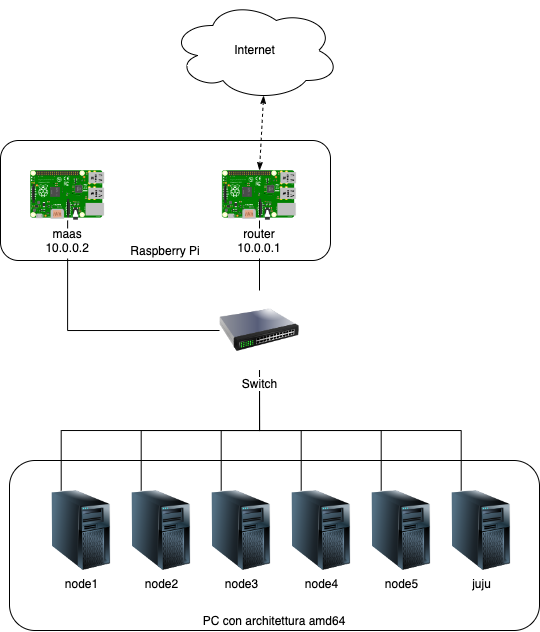
\includegraphics[scale=0.5]{tesi/files/immagini/network_architecture.png}
    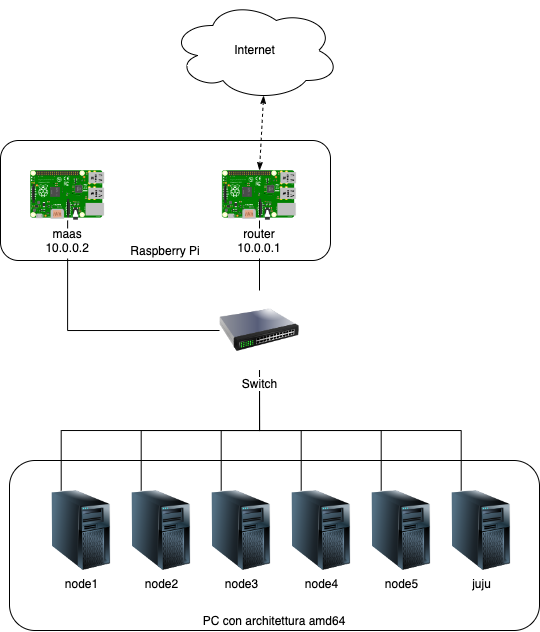
\includegraphics[width=0.8\linewidth]{tesi/files/immagini/network_architecture.png}
    \caption{Architettura di rete del cloud.}
    \label{fig:network_architecture}
\end{figure}

\noindent
Al Raspberry denominato nello schema \emph{router} è stato collegato l'adattatore ethernet USB, fornendogli un'interfaccia di rete aggiuntiva; in questo modo è stato possibile collegarlo ad internet.
% 
Il ruolo di questo Raspberry Pi è esclusivamente quello di comportarsi come un dispositivo di routing, connettendo così le due reti.
% 
La configurazione di questo dispositivo non verrà trattata in questo documento.

Il secondo Raspberry, denominato \emph{maas}, è quello su cui è stato installato l'intero sistema MAAS; la guida al deployment che è stata seguita prevedeva che MAAS fosse installato su una macchina simile a quelle utilizzate per il cloud ma, dopo un'attenta valutazione, è stato deciso di installarlo su un Raspberry Pi per avere una macchina aggiuntiva da dedicare a OpenStack.

Sul PC denominato \emph{juju} è stato installato il Juju Controller, ovvero il componente che gestisce e monitora tutti i charm che verranno installati sui nodi. 

I PC denominati \emph{nodeX} sono quelli dedicati al cloud vero e proprio, ovvero quelli su cui verranno installati tutti i componenti di OpenStack.

Inizialmente si era pensato di pianificare in quale macchina installare ciascun componente ma poi, dato che tutte le macchine sono uguali e che la guida di installazione non faceva distinzione tra le diverse macchine, si è deciso di non farlo. 
% 
Inoltre la quinta macchina è rimasta inutilizzata nel deployment iniziale ma si è rivelata fondamentale durante l'installazione del load balancer.



\subsection{Networking}\label{subsubsec:progettazione_networking}
Grazie alla modalità di deployment scelta, la configurazione della rete è molto semplice e gli indirizzi IP assegnati appartengono alla subnet \code{10.0.0.0/24}. 
% 
Come si può vedere dall'immagine in \cref{fig:network_architecture} ai Raspberry Pi \emph{router} e \emph{maas} sono stati assegnati rispettivamente gli indirizzi IP \code{10.0.0.1} e \code{10.0.0.2};
% 
le altre macchine invece non hanno indirizzi IP statici perché è il MAAS controller che si occupa di assegnarli al momento del deployment.

La scelta della subnet e degli indirizzi IP da assegnare a ciascuna macchina è totalmente arbitraria; 
% 
sono stati scelti questi perché sono gli stessi utilizzati nella guida all'installazione \cite{openstack_installation_juju}. 
% 
L'unico vincolo presente per la configurazione della rete è che almeno una delle subnet private di classe A rimanga inutilizzata; 
% 
questo perché LXD, durante l'inizializzazione automatica, sceglie tra queste subnet una da utilizzare per le proprie interfacce di rete virtuali e questa scelta viene fatta in base a quelle che non sono raggiungibili dalla macchina host \cite{lxd_init_network_error}. 
% 
Se questo vincolo non viene rispettato l'inizializzazione automatica di LXD fallisce e, anche nel caso in cui si tenti di farla manualmente, i container creati non saranno raggiungibili tramite rete.

Nelle fasi iniziale di questo progetto la rete era stata configurata sulla subnet \code{10.0.0.0/8} e questo, come si può intuire, ha causato non pochi problemi durante l'installazione dei charm su container perché l'inizializzazione di LXD stesso falliva senza dare messaggi di errore esplicativi.
% 
Il primo approccio di risoluzione è stato quello di inizializzare LXD manualmente;
% 
questo ha permesso di avviare i container contenenti i charm, ma è stato da subito chiaro che la comunicazione via rete non funzionasse correttamente.
% 
Dopo ulteriori tentativi e ricerche è stato possibile individuare il problema legato alla subnet e, dopo una riconfigurazione totale della rete, ha funzionato tutto come previsto.
